\documentclass[crop,tikz]{standalone}                 
\usepackage{physics}
\makeatletter                                                                                        

\begin{document}

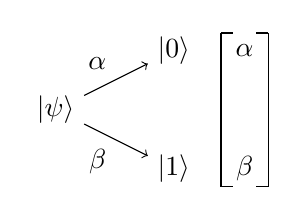
\begin{tikzpicture}[scale=1.5]                                                                          
%\draw [dotted] (0,0) grid (2, 1);
\node []   (nodeX) at ( 0.00,  0.50) {$\ket{\psi}$} ;                                           
\node []   (node0) at ( 1.00,  1.00) {$\ket{0}$}    ;                                          
\node []   (node1) at ( 1.00,  0.00) {$\ket{1}$}    ;    
\node []   (nodea) at ( 1.60,  1.00) {$\alpha$}     ;                                       
\node []   (nodeb) at ( 1.60,  0.00) {$\beta$}      ;                                       
\draw [->] (nodeX) -- (node0) node[midway, above left ] {$\alpha$};                                                           
\draw [->] (nodeX) -- (node1) node[midway, below left ] {$\beta$};                                                           
\draw [-]  ( 1.40,  1.15) -- (1.40, -0.15); %pillar                                                      
\draw [-]  ( 1.40, -0.15) -- (1.50, -0.15);                                                           
\draw [-]  ( 1.40,  1.15) -- (1.50,  1.15);                                                           
\draw [-]  ( 1.80,  1.15) -- (1.80, -0.15); %pillar                                                          
\draw [-]  ( 1.80, -0.15) -- (1.70, -0.15);                                                           
\draw [-]  ( 1.80,  1.15) -- (1.70,  1.15);   
\end{tikzpicture}                                                                                    

\end{document}
